%%mark = star, diamond, square, otimes
%\documentclass{article}
%\usepackage{pgfplots}
%\usepackage[justification=centering]{caption}
%\pgfplotsset{compat=newest}
%\begin{document}
\begin{figure}
\centering

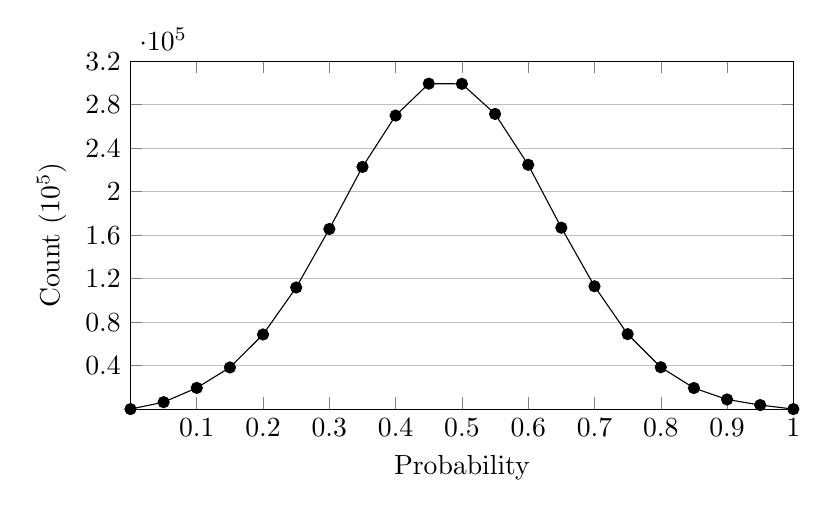
\begin{tikzpicture}
\begin{axis}[
 width=10cm,
   height=6cm,
    xlabel={Probability },
    ylabel={Count ($10^5$)},
    xmin=0, xmax=1.0,
    ymin=0, ymax=320000,
    xtick={.1,.2,.3,.4,.5,.6,.7,.8,.9,1.0},
    ytick={40000,80000,120000,160000,200000,240000,280000,320000},
    legend pos=north east,
    ymajorgrids=true,
    grid style={line width=.2pt,draw=gray!50},
]
 
\addplot[
    solid, every mark/.append style={solid, fill=black}, mark=*
    ]
    coordinates {
			(0,0)
			(0.05,6362)
			(0.1,19508)
			(0.15,38310)
			(0.2,68623)
			(0.25,111854)
			(0.3,165662)
			(0.35,222758)
			(0.4,269985)
			(0.45,299328)
			(0.5,299159)
			(0.55,271454)
			(0.6,224689)
			(0.65,166840)
			(0.7,112959)
			(0.75,68933)
			(0.8,38490)
			(0.85,19368)
			(0.9,8848)
			(0.95,3707)
			(1,0)
};
 
\end{axis}
\end{tikzpicture}
\caption{Probability Distribution for \emph{Pumsb Star} data set}
\label{result:data_pumsb_star}
\end{figure}
%\end{document}